\documentclass[conference]{IEEEtran}
\IEEEoverridecommandlockouts

% ---------- Paquetes ----------
\usepackage[spanish,es-tabla,es-noshorthands]{babel}
\usepackage[utf8]{inputenc}
\usepackage[T1]{fontenc}
\usepackage{cite}
\usepackage{amsmath,amssymb,amsfonts}
\usepackage{graphicx}
\graphicspath{{img/}}
\usepackage{textcomp}
\usepackage{xcolor}
\usepackage{booktabs}
\usepackage{tabularx}
\usepackage{array}
\usepackage{multirow}
\newcolumntype{Y}{>{\raggedright\arraybackslash}X}
\newcolumntype{P}[1]{>{\raggedright\arraybackslash}p{#1}}
\usepackage{url}
\usepackage{listings}
\usepackage{tikz}
\usetikzlibrary{positioning,arrows.meta,shapes.geometric,fit,calc}
% \FloatBarrier: evita que las figuras pasen a una fase posterior
\usepackage{placeins}
\usepackage{hyperref}

\hypersetup{colorlinks=true,linkcolor=blue,filecolor=magenta,urlcolor=cyan,citecolor=blue,
  pdftitle={Infraestructura de Red Local Autónoma para Atención Móvil Comunitaria en Entornos Rurales: Informe Final},
  pdfauthor={José David Rodríguez Pinilla, Carol Andrea Mosquera},
  pdfsubject={Infraestructura de Redes 2, Universidad Icesi},
  pdfkeywords={redes rurales, offline-first, portal cautivo, MikroTik, VLAN, Squid, Raspberry Pi 5, Starlink, CDN local}}

\lstset{
  basicstyle=\ttfamily\scriptsize,
  breaklines=true,
  breakatwhitespace=false,
  columns=fullflexible,
  keepspaces=true,
  frame=single,
  framerule=0.2pt,
  xleftmargin=2pt,xrightmargin=2pt,
  commentstyle=\itshape\color{gray},
  showstringspaces=false
}

\tikzset{
  box/.style={draw,rounded corners=2pt,align=center,font=\scriptsize,minimum height=7mm,fill=blue!5,inner sep=2pt},
  dev/.style={draw,rounded corners=2pt,align=center,font=\scriptsize,minimum height=7mm,fill=gray!10,inner sep=2pt},
  srv/.style={draw,thick,rounded corners=2pt,align=center,font=\scriptsize,minimum height=7mm,fill=green!8,inner sep=2pt},
  lnk/.style={-{Stealth[length=2mm]},thin},
  lbl/.style={font=\tiny,midway,fill=white,inner sep=1pt}
}

% Captura de evidencia a lo ancho de una columna
\newcommand{\evid}[3]{%
\begin{figure}[!htbp]\centering
\includegraphics[width=\columnwidth,height=0.25\textheight,keepaspectratio]{#1}
\caption{#2}\label{#3}
\end{figure}}

% Captura muy ancha (registros de terminal): a lo ancho de la página
\newcommand{\evidancha}[3]{%
\begin{figure*}[!t]\centering
\includegraphics[width=\textwidth,height=0.22\textheight,keepaspectratio]{#1}
\caption{#2}\label{#3}
\end{figure*}}

\begin{document}

\title{Infraestructura de Red Local Autónoma para Atención Móvil Comunitaria en Entornos Rurales: Informe Final}

\author{
\IEEEauthorblockN{José David Rodríguez Pinilla (A00407151) \quad Carol Andrea Mosquera (A00403934)}
\IEEEauthorblockA{\textit{Profesor: Andrés Navarro Cadavid, Ph.D.} \\
\textit{Infraestructura de Redes 2} \\
\textit{Departamento de Tecnologías de Información y Comunicaciones} \\
\textit{Universidad Icesi}, Cali, Colombia}
}

\maketitle

\begin{abstract}
Este informe presenta el diseño, la implementación y la evaluación experimental de una red local autónoma para una unidad móvil de atención comunitaria en zonas rurales. Las dos propuestas individuales de la Fase~1 se unificaron en un diseño consolidado: Starlink Mini como enlace WAN satelital, un enrutador MikroTik con RouterOS~7 en modo \textit{router-on-a-stick}, un punto de acceso con un SSID por VLAN y una Raspberry Pi~5 como servidor de servicios locales (``hub''), sobre el bloque \texttt{10.20.0.0/24} dividido con VLSM en tres VLAN: Administración (10), Salud (20) y Pública (30). El diseño se validó primero en un laboratorio virtual GNS3 y luego se llevó a hardware físico, un equipo a la vez: la Raspberry Pi física (2.1), el MikroTik CCR2004 (2.2), los servicios, el punto de acceso y el portal cautivo (2.3) y una CDN local de video (2.4). Funcionan el DHCP con relay, el DNS local con caché, la hora de red, el portal web con categorías y búsqueda local, la Wikipedia sin conexión por HTTPS, la caché HTTP transparente con Squid y conmutación automática, el portal cautivo por VLAN, el firewall entre VLAN, las colas de ancho de banda y el video a 720p sin conexión dentro del límite de 2~Mbps por usuario. Las 15 pruebas de red y las 4 de video se cumplieron. Con la Starlink conectada pero sin señal, todo el contenido local siguió disponible. Cada etapa se documenta con su procedimiento, sus decisiones, sus evidencias y los problemas resueltos, y se evalúa frente a los criterios de las tres fases de la rúbrica.
\end{abstract}

\begin{IEEEkeywords}
Redes rurales, offline-first, portal cautivo, MikroTik, RouterOS, VLAN 802.1Q, VLSM, Squid, Raspberry Pi 5, Starlink Mini, CDN local, HTTP Range Requests.
\end{IEEEkeywords}

%=====================================================================
\section{Introducción}
Una unidad móvil de atención comunitaria opera en zonas donde la conexión a Internet es escasa o costosa y la energía es inestable. Necesita una red propia que funcione con un enlace intermitente y también en aislamiento total. El enunciado pide un portal cautivo que dé a cada grupo de interés la experiencia de una red independiente con Internet, y un proxy/caché local sobre una Mini PC o una Raspberry Pi, con 2--4~TB de almacenamiento y funcionamiento completo sin conexión.

La red sigue la filosofía \textit{offline-first}: los servicios locales (portal, documentos, Wikipedia, videos educativos, DNS, DHCP, hora) no dependen de Internet, y el enlace satelital se usa para navegar y sincronizar cuando está disponible. La evaluación sigue una rúbrica de tres fases: plan de proyecto, prototipo funcional y sistema plenamente operacional.

\subsection{Metodología}
El trabajo avanzó de lo virtual a lo físico, cambiando un equipo a la vez, para que cada falla tuviera una sola causa posible. Después de cada cambio en el enrutador se guarda un \texttt{/export} con fecha y cada sesión termina con respaldos. Toda decisión o dato importante se registró el mismo día en un registro de decisiones del repositorio. La Tabla~\ref{tab:avance} resume la cronología; las secciones siguientes detallan cada etapa.

\begin{table*}[!t]
\centering
\caption{Cronología del proyecto y etapas de implementación}
\label{tab:avance}
\scriptsize
\begin{tabularx}{\textwidth}{llYl}
\toprule
\textbf{Etapa} & \textbf{Fecha} & \textbf{Resultado} & \textbf{Estado} \\
\midrule
1 Plan & 16--20/10/2026 & Dos versiones individuales del plan (José: informe IEEE con caché, almacenamiento, cronograma, presupuesto y riesgos; Carol: topología, VLSM, sumarización, rutas y matriz de tráfico) & Cumple \\
1 Consolidado & 20--26/10/2026 & Diseño único: MikroTik + Raspberry Pi 5 + Starlink Mini + UniFi, bloque \texttt{10.20.0.0/24} & Cumple \\
1.2 GNS3 & 26--27/10/2026 & MikroTik CHR 7.25 + Ubuntu Server 24.04.5: VLAN 10/20/30, NAT, DNS, clientes por VLAN y etiquetas 802.1Q verificadas & Cumple \\
2.1 RPi5 física & 30/10/2026 & La Raspberry Pi 5 física reemplaza a la VM del servidor y entra al laboratorio GNS3 por un nodo Cloud & Cumple \\
2.2 MikroTik físico & 05/11/2026 & CCR2004 prestado: respaldo del otro grupo, configuración del hub, portátil como WAN, pruebas 1--10 y restauración & Cumple \\
2.3 Servicios & 13--17/11/2026 & Pasos 1--6: ufw, SSH con llave, disco, dnsmasq + relay, chrony, Nginx HTTPS, Kiwix, Squid transparente, AP con dos SSID & Cumple \\
2.3 Portal y firewall & 18/11/2026 & Pasos 7--8: certificado, Hotspot, firewall entre VLAN y colas & Cumple \\
2.3 Rediseño y Starlink & 19/11/2026 & Portal con categorías y búsqueda, guías PDF, páginas del Hotspot en español, Starlink Mini integrada, pruebas P12/P13 y operación sin señal & Cumple \\
2.4 CDN de video & 20/11/2026 & Videos MP4 720p $\leq$1,2~Mbps con \textit{faststart} en \texttt{/srv/cdn/video/}, Nginx con peticiones de rango (206), catálogo \texttt{videos.html}; pruebas P1, P10 y V1--V4 & Cumple \\
\bottomrule
\end{tabularx}
\end{table*}

%=====================================================================
\section{Fase 1: plan de proyecto}

\subsection{Requisitos}
La Tabla~\ref{tab:req} resume los requisitos que se derivaron del enunciado en la Fase~1 y cómo los atiende el diseño vigente.

\begin{table}[!htbp]
\centering
\caption{Requisitos y cómo los atiende el diseño vigente}
\label{tab:req}
\scriptsize
\begin{tabularx}{\columnwidth}{lYY}
\toprule
\textbf{ID} & \textbf{Requisito} & \textbf{Diseño vigente} \\
\midrule
RQ1 & Red independiente con Internet cuando haya enlace & MikroTik con NAT hacia la Starlink Mini \\
RQ2 & Acceso diferenciado por grupo & Una VLAN, un SSID y un perfil de portal cautivo por grupo \\
RQ3 & Proxy local en Mini PC o Raspberry Pi & Squid transparente en la Raspberry Pi 5 \\
RQ4 & Almacenamiento de 2--4~TB & Disco USB~3 en \texttt{/srv/cdn} (ext4, \texttt{noatime}); SSD de 2~TB en la Fase~3 \\
RQ5 & Operar sin Internet & DNS, DHCP, hora, portal, Wikipedia y video locales \\
RQ6 & Tolerar cortes eléctricos & \texttt{nofail}, \texttt{RequiresMountsFor}, batería (Fase 3) \\
RQ7 & Proteger datos de salud & SSID WPA2 en VLAN propia, firewall, HTTPS sin descifrar \\
RQ8 & Contenido audiovisual fluido sin conexión & Nginx con peticiones de rango (206) y MP4 optimizado \\
\bottomrule
\end{tabularx}
\end{table}

\subsection{Versión de José}\label{sec:jose}
Plan en formato IEEE con la Raspberry Pi~5 como único nodo: enrutador (nftables), DHCP/DNS, portal cautivo (openNDS), proxy Squid y servidor de contenidos, sobre el bloque \texttt{10.10.0.0/16} (V10 Salud \texttt{/24}, V30 Portal \texttt{/23}, V99 Gestión \texttt{/28}) y un enlace LTE. Su principal aporte, que se mantiene, es la estrategia de caché y almacenamiento:
\begin{itemize}
\item Jerarquía de tres niveles: RAM (\texttt{cache\_mem}), NVMe para el sistema y objetos pequeños, y SSD de 2--4~TB para objetos grandes, ZIM de Kiwix y video.
\item Presupuesto del SSD de 2~TB: 200~GB de caché Squid, 1000~GB de video, 100~GB de Kiwix, 150~GB de cursos, 20~GB de PDF, 100~GB de respaldos y 15~\% de reserva.
\item Políticas \texttt{refresh\_pattern} por tipo de archivo, reemplazo \texttt{heap LFUDA} y HTTPS sin descifrar para no exponer datos de salud.
\item Cronograma de 11 semanas con ruta crítica, compras en tres lotes (USD~794 con 15~\% de contingencia) y una matriz de 12 riesgos; los de mayor nivel son el corte eléctrico (20), la falta de enlace (20) y la sobrecarga de trabajo (16).
\end{itemize}

\subsection{Versión de Carol}
Documento de topología, direccionamiento y enrutamiento con una Mini PC i5 como enrutador \textit{router-on-a-stick}, un router 4G y un túnel WireGuard (\texttt{172.31.255.0/30}) hacia un sitio central (\texttt{10.0.0.0/16}). Usa el bloque \texttt{10.20.0.0/22} con cuatro VLAN calculadas con VLSM a partir de la demanda con 50~\% de crecimiento: 30 Comunidad \texttt{/24}, 40 Invitados \texttt{/26}, 20 Personal \texttt{/27} y 10 Gestión \texttt{/28}, más un enlace \texttt{/30}. Desarrolla la sumarización (\texttt{/23} exacta, \texttt{/22} del sitio y \texttt{/20} multisitio), las tablas de rutas de cada equipo, los rangos DHCP y la matriz de tráfico permitido entre VLAN (Fig.~\ref{fig:carol}). De esta versión se mantienen el método VLSM, el prefijo \texttt{10.20} y la matriz de tráfico.

\begin{figure}[!htbp]
\centering
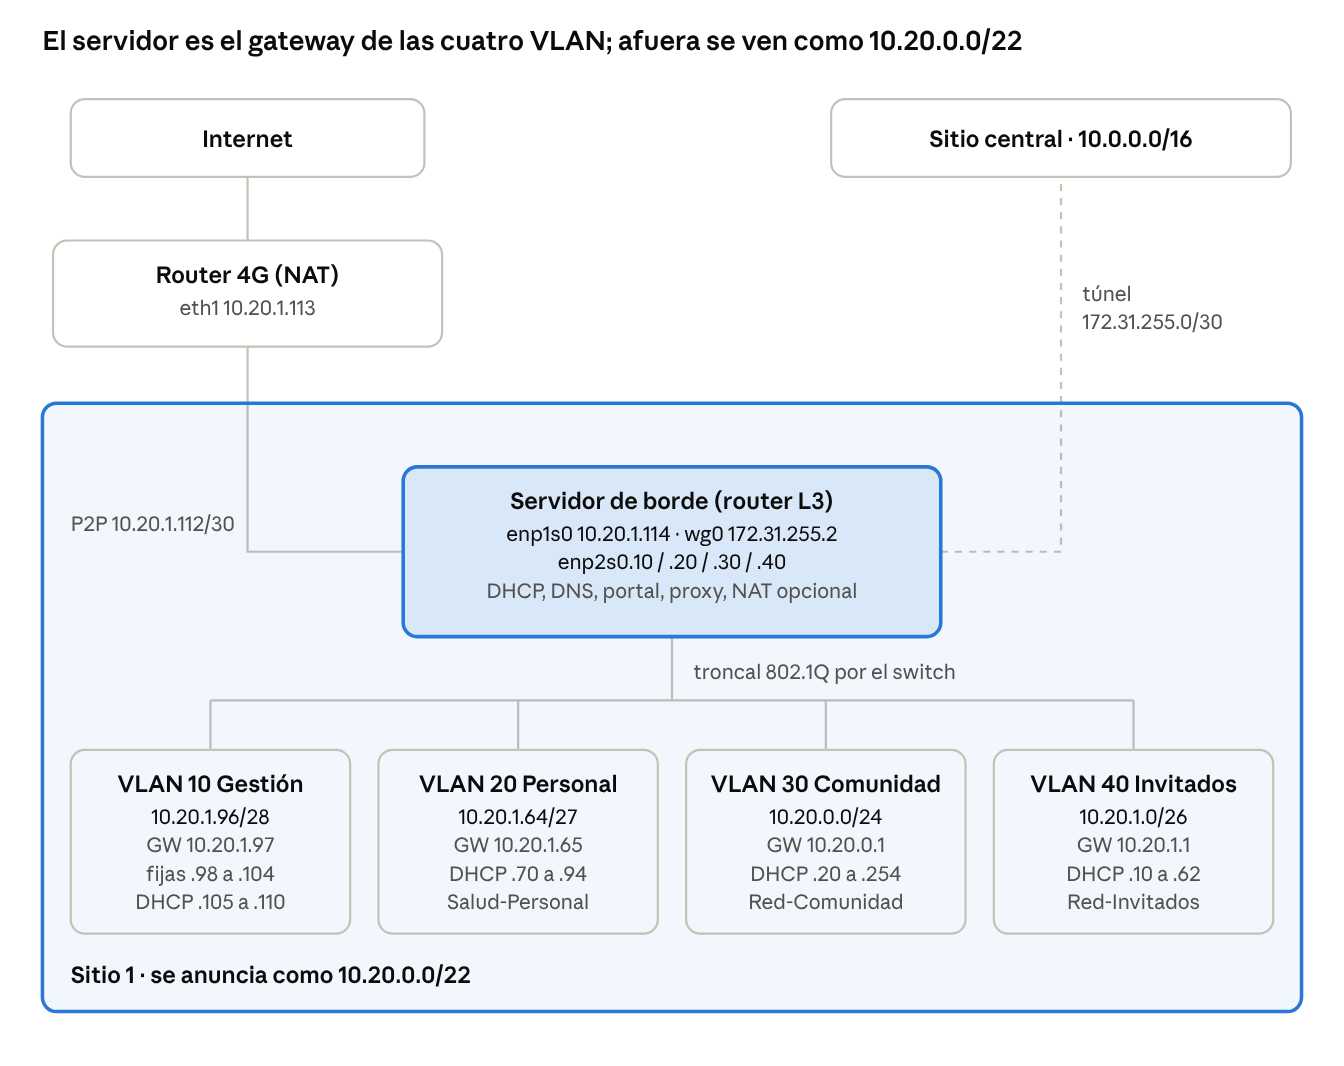
\includegraphics[width=\columnwidth]{f1-carol-topologia.png}
\caption{Topología lógica de la versión de Carol (Fase~1): servidor como gateway de cuatro VLAN, anunciadas como \texttt{10.20.0.0/22}.}
\label{fig:carol}
\end{figure}

\subsection{Diseño consolidado}
La Tabla~\ref{tab:versiones} compara ambas versiones con el diseño vigente. Separar el enrutamiento (MikroTik) de los servicios (Raspberry Pi) evita que una falla o una actualización del servidor deje sin red a los usuarios, y el MikroTik trae de fábrica el portal cautivo, las colas y el firewall. Se redujo el bloque a \texttt{/24}, suficiente para una sola unidad móvil, y se dejaron tres VLAN.

\begin{table*}[!t]
\centering
\caption{Versiones de la Fase~1 y diseño consolidado}
\label{tab:versiones}
\scriptsize
\begin{tabularx}{\textwidth}{lYYY}
\toprule
\textbf{Aspecto} & \textbf{Versión José} & \textbf{Versión Carol} & \textbf{Consolidado (vigente)} \\
\midrule
Enrutador L3 & Raspberry Pi 5 (nftables) & Mini PC i5 (router-on-a-stick) & MikroTik RouterOS 7 (router-on-a-stick) \\
Servidor & Raspberry Pi 5 & Mini PC i5 & Raspberry Pi 5 ``hub'', Ubuntu Server 24.04, IP fija en VLAN 10 \\
WAN & Router LTE & Router 4G + WireGuard & Starlink Mini (CGNAT) \\
Punto de acceso & Wi-Fi 6 genérico & 3 AP PoE & UniFi UAP-AC-M (en el laboratorio: TP-Link TL-WA801ND) \\
Portal cautivo & openNDS en la RPi5 & -- & Hotspot del MikroTik con páginas propias \\
Bloque & \texttt{10.10.0.0/16} & \texttt{10.20.0.0/22} & \texttt{10.20.0.0/24} \\
VLAN & 10 Salud, 30 Portal, 99 Gestión & 10 Gestión, 20 Personal, 30 Comunidad, 40 Invitados & 10 Administración, 20 Salud, 30 Pública \\
\bottomrule
\end{tabularx}
\end{table*}

%=====================================================================
\section{Arquitectura vigente}

\subsection{Equipos y topología}
La Fig.~\ref{fig:topo} muestra la topología. El MikroTik enruta las tres VLAN sobre un \textit{bridge} con \texttt{vlan-filtering}, hace NAT hacia la WAN, reenvía el DHCP al servidor (relay), desvía el HTTP a Squid y aplica el portal cautivo, el firewall y las colas. El punto de acceso asocia cada SSID a una VLAN y recibe una troncal 802.1Q~\cite{ieee8021q}. La Raspberry Pi~5 ``hub'' concentra los servicios locales.

\begin{figure}[!htbp]
\centering
\begin{tikzpicture}[node distance=6mm and 4mm]
 \node[dev] (inet) {Internet};
 \node[dev, below=of inet] (sl) {Starlink Mini\\(CGNAT)};
 \node[box, below=of sl, minimum width=40mm] (mk) {\textbf{MikroTik RouterOS 7}\\ \texttt{vlan10-admin} .161/28\\ \texttt{vlan20-salud} .129/27\\ \texttt{vlan30-publica} .1/25};
 \node[srv, below left=9mm and -6mm of mk] (hub) {Raspberry Pi 5\\``hub'' .162/28};
 \node[dev, below=9mm of mk] (ap) {Punto de acceso\\(SSID $\leftrightarrow$ VLAN)};
 \node[dev, below right=9mm and -6mm of mk] (adm) {Portátil\\admin};
 \node[dev, below left=7mm and -6mm of ap] (s20) {Hub-Salud\\VLAN 20};
 \node[dev, below right=7mm and -6mm of ap] (s30) {Hub-Publica\\VLAN 30};
 \draw[lnk] (inet) -- (sl);
 \draw[lnk] (sl) -- node[lbl]{WAN, DHCP} (mk);
 \draw (mk) -- node[lbl]{acceso V10} (hub);
 \draw (mk) -- node[lbl]{troncal} (ap);
 \draw (mk) -- node[lbl]{acceso V10} (adm);
 \draw (ap) -- (s20);
 \draw (ap) -- (s30);
\end{tikzpicture}
\caption{Topología del diseño consolidado. Troncal del AP: VLAN 10 sin etiqueta, VLAN 20 y 30 etiquetadas.}
\label{fig:topo}
\end{figure}

\subsection{Direccionamiento y DHCP}
El bloque \texttt{10.20.0.0/24} (RFC~1918~\cite{rfc1918}) se divide con VLSM según la demanda de cada grupo (Tabla~\ref{tab:vlsm}). Quedan libres \texttt{10.20.0.176/28} y \texttt{10.20.0.192/26} para crecer. El NAT es \texttt{srcnat 10.20.0.0/24} $\rightarrow$ WAN \texttt{masquerade}; con el CGNAT de Starlink hay doble traducción, de modo que desde Internet no se pueden iniciar conexiones hacia el sitio. El DHCP lo da la Raspberry para las tres VLAN; las concesiones son cortas donde rotan más usuarios.

\begin{table}[!htbp]
\centering
\caption{VLSM sobre \texttt{10.20.0.0/24} y rangos DHCP}
\label{tab:vlsm}
\scriptsize
\begin{tabular}{llllll}
\toprule
\textbf{VLAN} & \textbf{Uso} & \textbf{Subred} & \textbf{GW} & \textbf{DHCP} & \textbf{Conc.} \\
\midrule
10 & Admin. & \texttt{.160/28} & \texttt{.161} & \texttt{.170--.174} & 24 h \\
20 & Salud & \texttt{.128/27} & \texttt{.129} & \texttt{.135--.158} & 8 h \\
30 & Pública & \texttt{.0/25} & \texttt{.1} & \texttt{.10--.126} & 30 min \\
\bottomrule
\end{tabular}
\end{table}

En la VLAN~10 hay direcciones fijas: \texttt{.161} MikroTik, \texttt{.162} Raspberry, \texttt{.163} punto de acceso y \texttt{.164--.169} reservadas.

\subsection{Matriz de tráfico}
La Tabla~\ref{tab:matriz} es la política que aplica el firewall del MikroTik (Sección~\ref{sec:f23}). Se basa en la matriz de tráfico de la versión de Carol.

\begin{table}[!htbp]
\centering
\caption{Tráfico permitido por origen}
\label{tab:matriz}
\scriptsize
\begin{tabularx}{\columnwidth}{lYYll}
\toprule
\textbf{Origen} & \textbf{MikroTik} & \textbf{Raspberry} & \textbf{Otras VLAN} & \textbf{Internet} \\
\midrule
VLAN 10 & SSH, WinBox & Todo & Sí & Sí \\
VLAN 20 & DHCP, DNS, portal & DNS, NTP, HTTP(S), MQTT & No & Tras sesión \\
VLAN 30 & DHCP, DNS, portal & DNS, NTP, HTTP(S) & No & Tras portal \\
Internet & No & No & -- & -- \\
\bottomrule
\end{tabularx}
\end{table}

\subsection{Puertos del enrutador}
El plan usa \texttt{ether1}--\texttt{ether4}. En el laboratorio físico se usó un MikroTik prestado con otros números de puerto, pero la lógica es la misma (Tabla~\ref{tab:puertos}).

\begin{table}[!htbp]
\centering
\caption{Puertos del MikroTik en cada etapa}
\label{tab:puertos}
\scriptsize
\begin{tabularx}{\columnwidth}{YlllY}
\toprule
\textbf{Rol} & \textbf{Plan} & \textbf{GNS3} & \textbf{CCR2004} & \textbf{Modo} \\
\midrule
WAN & ether1 & ether1 & ether9 & DHCP, fuera del \textit{bridge} \\
Raspberry & ether2 & ether2 & ether10 & Acceso V10 \\
Punto de acceso & ether3 & ether3 & ether11 & Troncal 10/20/30 \\
Portátil admin & ether4 & ether4 & ether12 & Acceso V10 \\
\bottomrule
\end{tabularx}
\end{table}

%=====================================================================
\section{Fase 1.2: laboratorio virtual en GNS3}
Antes de usar hardware, el diseño se montó en GNS3 2.2.61 sobre Ubuntu con el mismo software de los equipos reales, para validar las capas 2 y 3. Se eligió Ubuntu en vez de Windows porque GNS3 corre las máquinas directo sobre KVM, sin la virtualización anidada de la GNS3~VM.

La topología (Fig.~\ref{fig:gns3}) tiene un nodo NAT que hace de Starlink, un MikroTik CHR~7.25, una VM Ubuntu Server 24.04.5 como servidor, un switch de GNS3 que simula el AP (puerto 0 \texttt{dot1q} con nativa 10, puerto 1 VLAN 20, puerto 2 VLAN 30) y tres clientes livianos (Alpine Linux y dos webterm con Firefox) que hacen de portátil y teléfonos. El orden de montaje fue: NAT, MikroTik, switch, servidor y clientes, porque cada paso necesita al anterior.

\evid{f12-gns3-topologia.png}{Topología del laboratorio GNS3: Starlink-NAT, MikroTik CHR, AP simulado, servidor Ubuntu y clientes de cada VLAN.}{fig:gns3}

La Fig.~\ref{fig:chr} muestra el MikroTik con las VLAN 10, 20 y 30 en el \textit{bridge}, las tres direcciones de gateway y las rutas, y la Fig.~\ref{fig:srv12} al servidor llegando al gateway, a Internet y al DNS.

\evid{f12-chr-vlan-direcciones.png}{MikroTik CHR: VLAN del \textit{bridge}, direcciones, rutas y \texttt{/export} guardado como \texttt{hub-base}.}{fig:chr}

\evid{f12-servidor-pruebas.png}{Servidor virtual en \texttt{10.20.0.162/28}: ping al gateway, a \texttt{8.8.8.8} y a \texttt{ubuntu.com}.}{fig:srv12}

\subsection{Pruebas}
El 27/10/2026 se cumplieron: salida a Internet del MikroTik, VLAN en el \textit{bridge}, servidor con su IP fija, gateway, Internet y DNS desde el servidor, \texttt{apt} con \texttt{archive.ubuntu.com}, puertos del switch, WebFig del gateway, navegación desde los clientes de salud y pública, y las pruebas A1--A11 del cliente de administración. Las etiquetas 802.1Q se verificaron en Wireshark. El aislamiento entre VLAN quedó para la Fase~2, porque requiere el firewall. Se guardó el \texttt{/export} en \texttt{hub-base.rsc}.

\subsection{Problemas resueltos}
Se registraron 15 problemas del montaje (26--27/10). Los más relevantes:
\begin{itemize}
\item \textbf{uBridge no disponible:} el usuario se agregó al grupo, pero la sesión era anterior; se resolvió reiniciando.
\item \textbf{Disco del MikroTik dañado:} un cierre inesperado de GNS3 dañó el \texttt{qcow2}; se recreó el nodo y se volvió a aplicar el script en un minuto. Lección: \texttt{/export} después de cada cambio.
\item \textbf{Mirror de Ubuntu sin respuesta:} el espejo de Colombia (\texttt{co.archive.ubuntu.com}) no respondía; se usó el principal, \texttt{archive.ubuntu.com}.
\item \textbf{Clientes webterm sin red:} el contenedor arranca sin configuración; se fijó la IP según la VLAN del puerto.
\end{itemize}

%=====================================================================
\section{Fase 2.1: Raspberry Pi 5 física}
Primera etapa del paso a lo físico (30/10/2026): la Raspberry Pi~5 reemplaza a la VM del servidor, conectada por cable al portátil y unida al MikroTik virtual con un nodo Cloud de GNS3 (Fig.~\ref{fig:cloud}).

\begin{enumerate}
\item Se grabó Ubuntu Server 24.04 LTS de 64 bits con Raspberry Pi Imager (hostname \texttt{hub}, zona \texttt{America/Bogota}, SSH, sin WiFi) y se alimentó con la fuente oficial de 27~W.
\item Se actualizó el sistema y se reinició para cargar el kernel \texttt{6.8.0-1065}.
\item Se apagó la VM del servidor para no duplicar \texttt{10.20.0.162}.
\item Se deshabilitó la red de cloud-init, que podía reescribir la configuración en un reinicio, y se creó \texttt{/etc/netplan/01-hub.yaml} con la IP fija (Fig.~\ref{fig:rpiip}).
\item El puerto Ethernet del portátil se dejó sin IPv4 ni IPv6, para que funcione solo como cable. Si quedaba en modo ``Compartida'' habría un segundo DHCP y un segundo gateway (\texttt{10.42.0.1}) dentro de la VLAN~10, y las pruebas de firewall, colas y portal darían resultados falsos.
\end{enumerate}

\evid{f21-gns3-nodo-cloud.png}{GNS3 con el nodo Cloud \texttt{rasberryFisica} (\texttt{enp46s0}) conectado a \texttt{ether2} del MikroTik.}{fig:cloud}

\evid{f21-rpi-ip-fija.png}{Consola de la Raspberry física: \texttt{eth0} con \texttt{10.20.0.162/28}.}{fig:rpiip}

Las pruebas (ping al gateway, a Internet y por nombre, SSH desde el cliente Alpine y desde el portátil, \texttt{apt update} y hora sincronizada) se cumplieron (Fig.~\ref{fig:rpiapt}).

\evid{f21-rpi-apt-hora.png}{Raspberry física: \texttt{apt update} sin errores y reloj sincronizado en \texttt{America/Bogota}.}{fig:rpiapt}

%=====================================================================
\FloatBarrier
\section{Fase 2.2: MikroTik físico}
Segunda etapa (05/11/2026): el MikroTik deja de ser virtual y la Raspberry se conecta directo a él. Se usó un CCR2004-16G-2S+ con RouterOS 7.13.5 (\texttt{sw01}) que pertenece a otro grupo, así que cada sesión empieza respaldando su configuración y termina restaurándola.

\subsection{Procedimiento}
\begin{itemize}
\item \textbf{A. Respaldo del otro grupo:} \texttt{/system backup save} y \texttt{/export show-sensitive} con la fecha. El portátil entró temporalmente a la VLAN~10 del otro grupo con una IP dentro de su rango SSH permitido, descargó los archivos por \texttt{scp}, los verificó y envió un ZIP con una nota de restauración (Fig.~\ref{fig:resp}).
\item \textbf{B. Puertos:} el hub usa \texttt{ether9}--\texttt{ether12}, que el otro grupo tiene deshabilitados, para no mover sus cables; el resto queda deshabilitado (Figs.~\ref{fig:puertos} y~\ref{fig:foto22}).
\item \textbf{C. Configuración:} reset sin valores de fábrica y pegado por consola serial en cinco bloques: identidad y hora, puertos, \textit{bridge} y VLAN, direcciones/DHCP-client/DNS/NAT/NTP y servicios de gestión (solo SSH, WinBox y WebFig).
\item \textbf{D. Portátil como WAN:} el portátil comparte su WiFi por el cable hacia \texttt{ether9} (red \texttt{10.42.0.0/24}), igual que la Starlink o el nodo NAT de GNS3 (Fig.~\ref{fig:wan}).
\item \textbf{E. Cierre:} respaldo del hub, carga del respaldo del otro grupo y borrado de los archivos propios (Fig.~\ref{fig:rest}).
\end{itemize}

\evid{f22-respaldo-otro-grupo.png}{Respaldo \texttt{sw01-original-2026-11-05} de la configuración del otro grupo antes de resetear el equipo.}{fig:resp}

\evid{f22-puertos-ccr2004.png}{Puertos del CCR2004 con la configuración del hub: solo \texttt{ether9}--\texttt{ether12} habilitados, con su función en el comentario.}{fig:puertos}

\evid{f22-foto-ccr2004.png}{CCR2004 del laboratorio con los cables del hub en \texttt{ether9} y \texttt{ether10}.}{fig:foto22}

\evid{f22-wan-dhcp-ping.png}{\texttt{ether9} recibe \texttt{10.42.0.116/24} del portátil; el MikroTik llega a \texttt{8.8.8.8} y resuelve \texttt{google.com}.}{fig:wan}

\subsection{Pruebas}
Se cumplieron las 10 pruebas: enlaces activos solo en los puertos del hub, cliente DHCP en \texttt{bound}, ping a Internet y a la Raspberry, MAC de la Raspberry en la VLAN~10, Raspberry hacia el gateway, Internet y DNS (Fig.~\ref{fig:rpi22}), \texttt{apt update}, SSH a los dos equipos y contador del NAT en aumento.

\evid{f22-rpi-pruebas.png}{Raspberry conectada directo al MikroTik físico: ping al gateway, a \texttt{8.8.8.8} y a \texttt{ubuntu.com}.}{fig:rpi22}

\evid{f22-restauracion.png}{Restauración de la configuración del otro grupo al terminar la sesión.}{fig:rest}

\subsection{Problemas resueltos}
\begin{itemize}
\item Caracteres perdidos al pegar por consola serial: se pega por bloques y se revisa cada resultado.
\item \texttt{scp} al equipo del otro grupo sin respuesta: la IP del portátil estaba fuera de su rango SSH permitido.
\item \texttt{REMOTE HOST IDENTIFICATION HAS CHANGED} al entrar a la Raspberry: huella de la VM anterior; se borró con \texttt{ssh-keygen -R}.
\end{itemize}

%=====================================================================
\FloatBarrier
\section{Fase 2.3: servicios, punto de acceso y portal cautivo}\label{sec:f23}
Tercera etapa, hecha en varias sesiones entre el 13 y el 19/11/2026 (Fig.~\ref{fig:montaje}). El orden importa: el punto de acceso va después del DHCP, porque sin él los celulares se conectan pero no reciben dirección, y el portal cautivo va después del DNS y del certificado.

\evid{f23-foto-montaje.png}{Montaje de la Fase 2.3: CCR2004, Raspberry Pi~5 y disco USB.}{fig:montaje}

\textbf{Decisión de despliegue:} en el prototipo los servicios se instalan con \texttt{apt} y corren con systemd, sin Docker. Así gastan menos RAM, arrancan sin depender de otro servicio y \texttt{RequiresMountsFor=/srv/cdn} impide que arranquen si falta el disco.

\subsection{Paso 1: seguridad y disco de la Raspberry}
\begin{itemize}
\item Actualizaciones de seguridad automáticas con el paquete \texttt{unattended-upgrades}.
\item ufw con política \textit{deny} de entrada; solo se abren SSH desde la VLAN~10, DNS, DHCP, NTP, HTTP/HTTPS y Squid hacia \texttt{10.20.0.0/24}, más una regla del portátil solo para el laboratorio (Fig.~\ref{fig:ufw}).
\item SSH solo con llave, sin \texttt{root} y solo para el usuario \texttt{carol}.
\item Disco USB de 465~GB revisado con SMART antes de usarlo (Fig.~\ref{fig:smart}), formateado en ext4 con 1~\% de reserva y un inodo cada 64~KiB (archivos grandes), y montado en \texttt{/srv/cdn} con \texttt{noatime,nofail} (Fig.~\ref{fig:disco}). \texttt{noatime} evita una escritura por cada lectura; \texttt{nofail} deja arrancar la Raspberry aunque el disco falle, para que el DNS y el DHCP sigan funcionando.
\end{itemize}

\evid{f23-ufw.png}{Reglas de ufw: solo los servicios del hub y solo hacia su red.}{fig:ufw}

\evid{f23-smart-disco.png}{Salud del disco usado: SMART \texttt{PASSED} y cero sectores reasignados, pendientes o incorregibles.}{fig:smart}

\evid{f23-disco-srv-cdn.png}{Formato del disco, línea de \texttt{/etc/fstab} y montaje en \texttt{/srv/cdn} con \texttt{noatime}.}{fig:disco}

\subsection{Paso 2: DNS y DHCP con relay}
dnsmasq~\cite{dnsmasq} escucha solo en \texttt{eth0}, responde el dominio local \texttt{hub.lan} (\texttt{portal}, \texttt{cdn}, \texttt{wiki}, \texttt{mikrotik}, \texttt{ap}) aunque no haya Internet, pregunta afuera a \texttt{1.1.1.1} y \texttt{9.9.9.9} y guarda 10\,000 respuestas en caché, de modo que lo repetido no gasta enlace satelital. Entrega los tres rangos de la Tabla~\ref{tab:vlsm} con el gateway de cada red y la Raspberry como DNS y servidor de hora. Como la Raspberry solo está en la VLAN~10, el MikroTik reenvía las peticiones de las VLAN 20 y 30 con un relay por VLAN (Fig.~\ref{fig:relay}); el \texttt{local-address} le indica a dnsmasq de qué red viene cada pedido.

\evid{f23-relay-dhcp.png}{Relay DHCP en el MikroTik hacia \texttt{10.20.0.162}: \texttt{relay-salud} y \texttt{relay-publica}.}{fig:relay}

\subsection{Paso 3: hora de red}
chrony toma la hora de Internet cuando hay conexión y la sigue dando sin ella (\texttt{local stratum 10}). El MikroTik dejó \texttt{pool.ntp.org} y se sincroniza con la Raspberry (Fig.~\ref{fig:ntp}); los celulares la reciben por DHCP. Sin hora correcta, los certificados HTTPS fallan.

\evid{f23-ntp-sincronizado.png}{Cliente NTP del MikroTik \texttt{synchronized} con \texttt{10.20.0.162}.}{fig:ntp}

\subsection{Paso 4: contenido por HTTPS}
Se creó una CA de pruebas y, con ella, un certificado comodín \texttt{*.hub.lan} de 365 días (los navegadores rechazan los de más de 398), válido para el portal, la CDN, la wiki y las páginas del portal cautivo (Fig.~\ref{fig:cert}). Nginx~\cite{nginx} redirige todo el HTTP a HTTPS, salvo la descarga de la CA y su guía de instalación; sirve el portal, sitios educativos copiados con \texttt{wget --mirror}, documentos PDF con listado automático y caché de 30 días en el celular, y pone HTTPS delante de Kiwix~\cite{kiwix}, que sirve una Wikipedia en español sin conexión solo en \texttt{127.0.0.1:8080}.

\evid{f23-certificado.png}{Certificado \texttt{*.hub.lan} emitido por la CA de pruebas, con \texttt{DNS:hub.lan}, \texttt{DNS:*.hub.lan} e \texttt{IP:10.20.0.162}.}{fig:cert}

\subsection{Paso 5: caché Squid y desvío transparente}
Squid~\cite{squid} guarda lo que se descarga por HTTP, así la segunda persona que lo pide no gasta otra vez el enlace. Solo la red del hub puede usarlo. Usa 256~MB de RAM, objetos de hasta 512~MB, reemplazo \texttt{heap LFUDA}, \texttt{refresh\_pattern} largos para instaladores, PDF y video, y 4~GB de caché en disco mientras llega el SSD definitivo (unos 50~GB en una Pi de 4~GB de RAM, porque Squid usa unos 10~MB de RAM por GB de caché). El HTTPS sale directo: no se descifra, para no exponer datos de salud ni obligar a instalar certificados falsos.

El MikroTik marca el HTTP de las VLAN 20 y 30 hacia Internet (regla \texttt{pbr-squid}) y lo envía por la tabla \texttt{to-proxy}, cuya única salida es la Raspberry; allí iptables lo pasa al puerto \texttt{3129 intercept} (Fig.~\ref{fig:pbr}). Hay dos protecciones: \texttt{check-gateway=ping} desactiva la ruta si la Raspberry no responde, y un \textit{netwatch} desactiva la regla si Squid se cae. En ambos casos se pierde la caché, no la navegación. La Fig.~\ref{fig:squidlog} muestra un celular de Hub-Publica pasando por Squid.

\evid{f23-pbr-squid.png}{Tabla \texttt{to-proxy}, ruta hacia la Raspberry, regla \texttt{pbr-squid} y \textit{netwatch} en el MikroTik.}{fig:pbr}

\evidancha{f23-squid-log.png}{Registro de Squid: tráfico del celular \texttt{10.20.0.64} con \texttt{TCP\_MISS} y \texttt{TCP\_HIT}.}{fig:squidlog}

\subsection{Paso 6: punto de acceso}
El prototipo usa el TP-Link TL-WA801ND del laboratorio; el UniFi UAP-AC-M sigue siendo el del diseño final, con la misma configuración SSID$\leftrightarrow$VLAN. Se respaldó su configuración original, se desactivó su DHCP, se activó Multi-SSID con VLAN (Hub-Salud en la 20 con WPA2-PSK AES; Hub-Publica en la 30, abierta porque el control lo hace el portal) y se le dio la IP fija \texttt{10.20.0.163} (Fig.~\ref{fig:tplink}). No se creó SSID de administración: la VLAN~10 viaja sin etiqueta en la troncal y la gestión se hace por cable. El AP se conectó a \texttt{ether11} (Fig.~\ref{fig:fotoap}) y responde desde el MikroTik (Fig.~\ref{fig:pingap}).

\evid{f23-tplink-multissid.png}{TP-Link en Multi-SSID con VLAN: Hub-Salud en la VLAN 20 y Hub-Publica en la VLAN 30.}{fig:tplink}

\evid{f23-foto-ap.png}{Punto de acceso TP-Link TL-WA801ND conectado a la troncal \texttt{ether11}.}{fig:fotoap}

\evid{f23-ping-ap.png}{\texttt{ether11} activo y ping del MikroTik al punto de acceso \texttt{10.20.0.163}.}{fig:pingap}

Con un celular se comprobó que aparecen los dos SSID y que cada red entrega una IP de su rango por el relay (Fig.~\ref{fig:cel}). Después se instaló la CA de pruebas en el celular y \texttt{https://portal.hub.lan} abrió con candado.

\begin{figure}[!htbp]
\centering
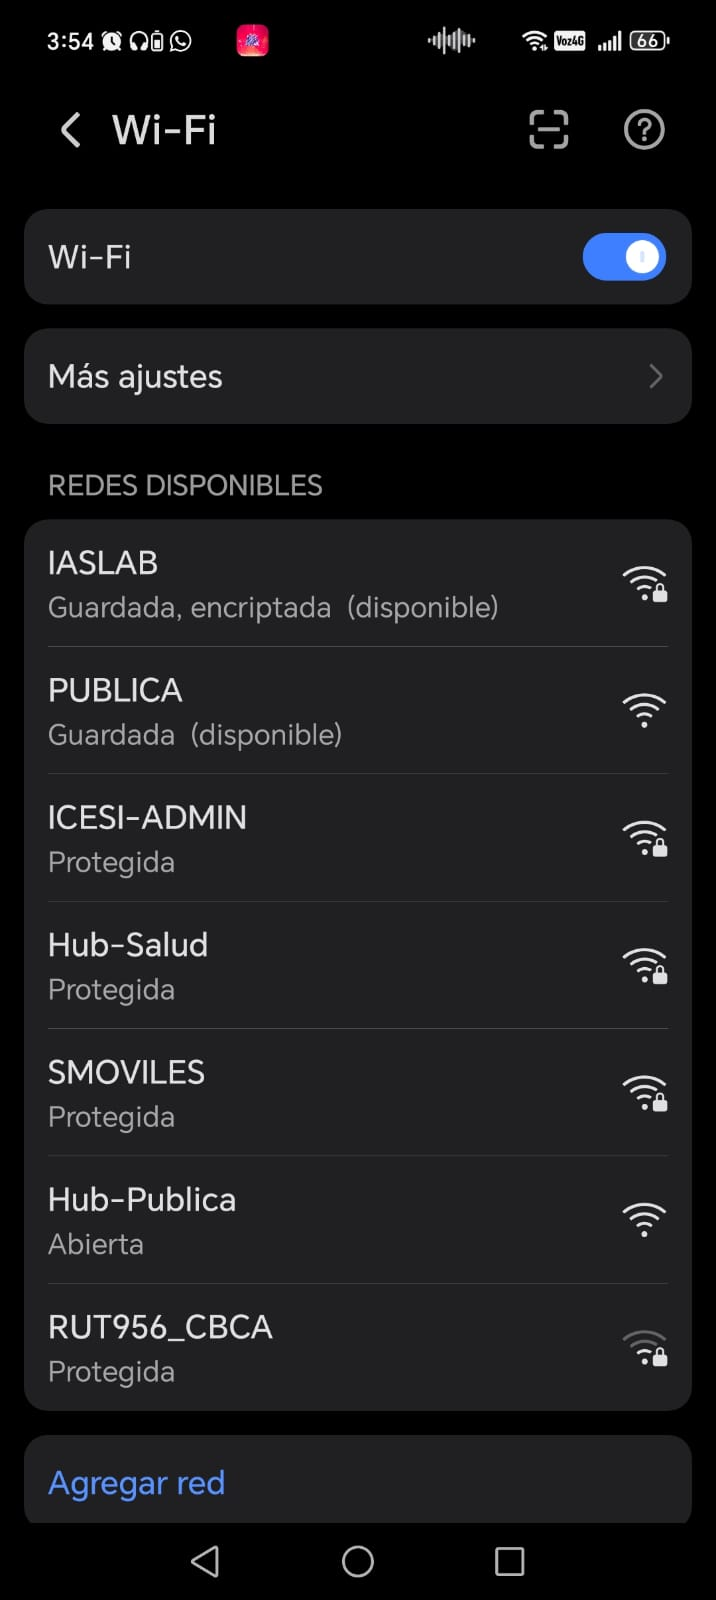
\includegraphics[width=0.32\columnwidth]{f23-celular-ssid.png}\hfill
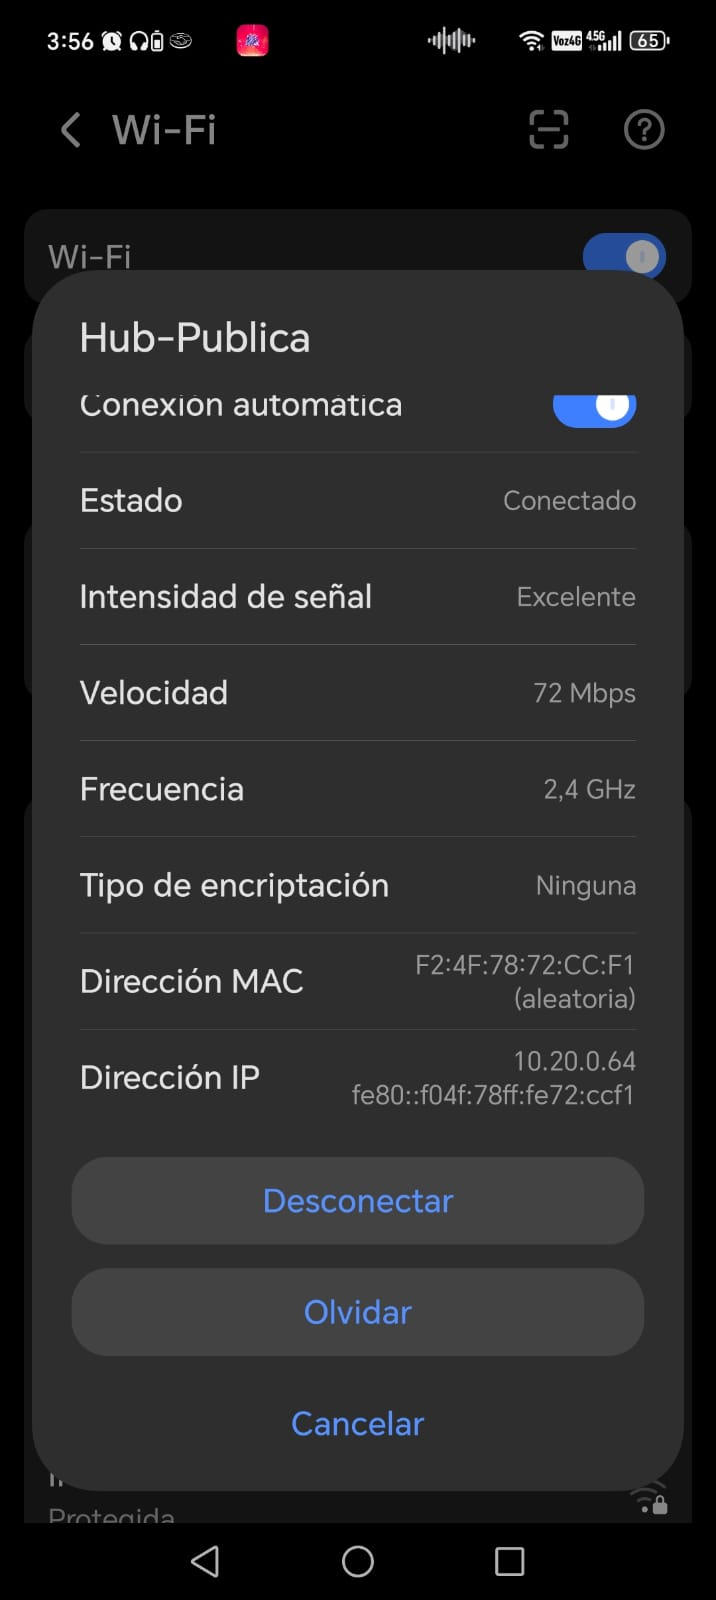
\includegraphics[width=0.32\columnwidth]{f23-celular-publica.png}\hfill
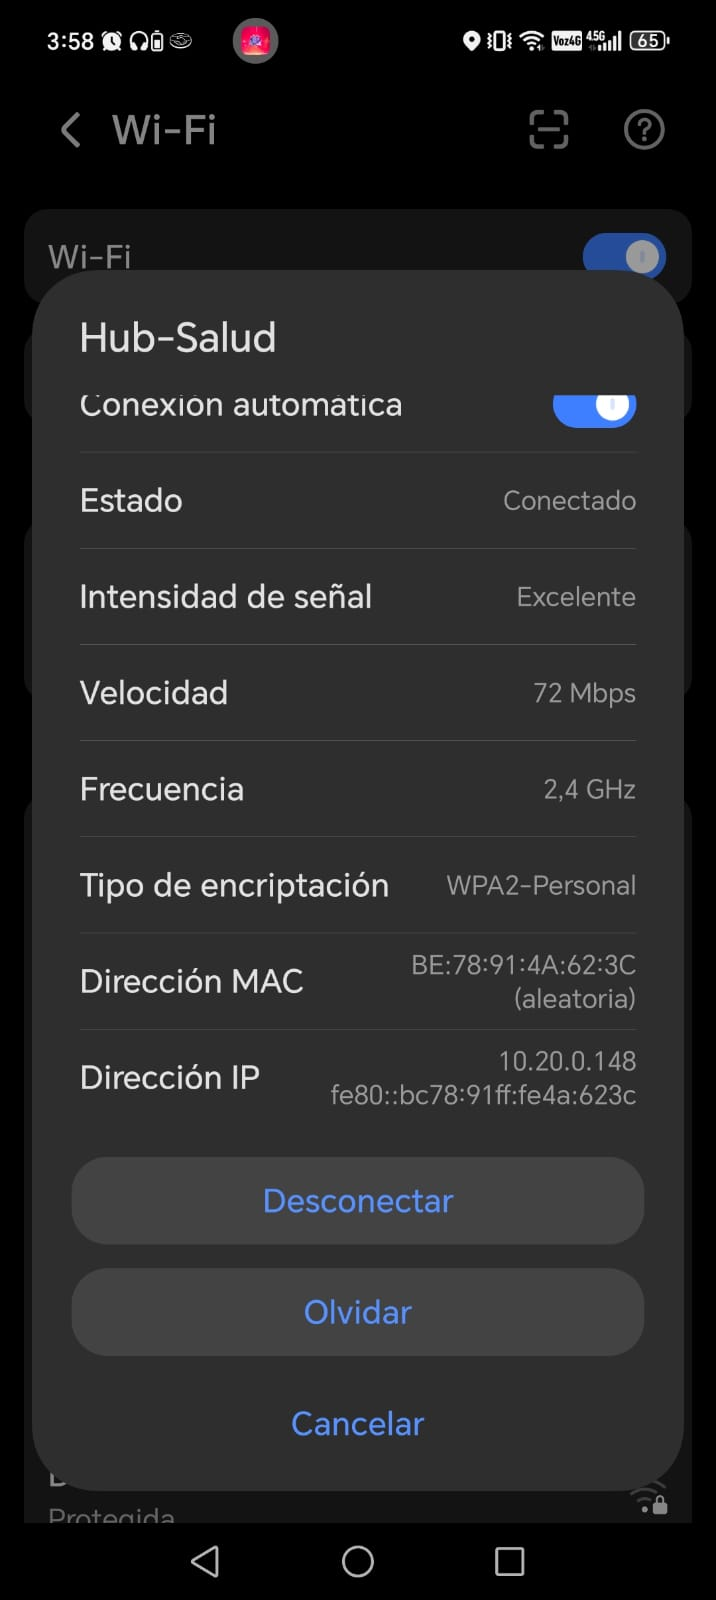
\includegraphics[width=0.32\columnwidth]{f23-celular-salud.png}
\caption{Celular: (izq.) SSID Hub-Salud (protegida) y Hub-Publica (abierta); (centro) \texttt{10.20.0.64} por relay en Hub-Publica; (der.) \texttt{10.20.0.148} en Hub-Salud.}
\label{fig:cel}
\end{figure}

\subsection{Paso 7: portal cautivo}
El portal lo hace el Hotspot del MikroTik, porque es la puerta de enlace de las VLAN y decide quién sale a Internet. El certificado \texttt{*.hub.lan} se importó al MikroTik y la copia temporal de la llave se borró de los tres equipos.
\begin{itemize}
\item \textbf{Hub-Publica} (\texttt{wifi-publica.hub.lan}): el portal aparece solo, ofrece ``Ver contenido sin conexión'' sin iniciar sesión y una prueba gratuita de 2~h a 1/2~Mbps.
\item \textbf{Hub-Salud} (\texttt{wifi-salud.hub.lan}): pide usuario y clave, guardados en el MikroTik para que funcione sin Internet; sesiones de 8~h, dos dispositivos por usuario.
\item Las dos páginas van por HTTPS. El Hotspot no reparte IP (lo sigue haciendo dnsmasq por relay) y la Raspberry está en el \textit{walled garden}, así que el contenido local se ve sin iniciar sesión. El desvío a Squid solo actúa sobre usuarios que ya pasaron el portal.
\end{itemize}

\subsection{Paso 8: firewall y colas}
El firewall tiene 18 reglas sobre las listas \texttt{LAN}/\texttt{WAN} que aplican la Tabla~\ref{tab:matriz}: aceptar respuestas, descartar inválidos, gestión solo desde la VLAN~10, DNS y relay DHCP hacia el MikroTik, DNS/NTP/HTTP/HTTPS hacia la Raspberry, MQTT (8883) reservado para la VLAN~20, HTTP desviado a Squid, salida a Internet y descarte de todo lo demás, incluido el tráfico entre VLAN. Dos reglas son solo del laboratorio (gestión desde el portátil) y se borran con la WAN definitiva. Se aplicó por SSH con un \texttt{/system scheduler} que borraba las reglas a los 5~min si se perdía el acceso, y se canceló al comprobar que todo funcionaba.

Las colas aplican los valores de la Fase~1: \texttt{salud} con 3/10~Mbps garantizados y prioridad~1; \texttt{publica} con un máximo de 5/20~Mbps para todo el grupo y, dentro de ella, una cola de 1/2~Mbps (subida/bajada) por usuario creada por el Hotspot. Con 50 usuarios públicos, cada uno tiene al menos 0,4~Mbps. Se ajustarán al medir la velocidad real de la Starlink.

\subsection{Contenido sin conexión, guías y portal}
El 18/11 se aplicaron los pasos 7 y 8 sobre el respaldo del 17/11 y se comprobó, comparando los \texttt{/export}, que el \textit{bridge}, las VLAN, los puertos, las IP, el relay, el NAT y el desvío a Squid no cambiaron: solo hubo líneas agregadas.

El 19/11 se agregaron nueve documentos en las tres categorías del portal (\texttt{pdf/salud}, \texttt{pdf/educacion} y \texttt{pdf/ocio}): cinco artículos de Wikipedia en español exportados a PDF (licencia CC~BY-SA) y cuatro guías propias generadas con scripts en Python: lavado de manos según la OMS~\cite{who-hh}, primeros auxilios según la IFRC~\cite{ifrc-fa}, una cartilla de matemáticas con ejemplos rurales y respuestas verificadas por el propio script, y ocho fábulas de Samaniego, de dominio público, tomadas de Wikisource. Cada guía de salud lleva el aviso de llamar al 123 y su lista de referencias (Figs.~\ref{fig:guias} y~\ref{fig:pdfs}). La Wikipedia sin conexión responde por HTTPS y su búsqueda devuelve artículos (Fig.~\ref{fig:kiwix}).

\evid{f23-guias-pdf.png}{Portadas de las guías propias: lavado de manos, primeros auxilios, cartilla de matemáticas y fábulas de Samaniego.}{fig:guias}

\evid{f23-pdf-categorias.png}{Documentos en \texttt{/srv/cdn/www/pdf/} por categoría, servidos por HTTPS como \texttt{application/pdf}.}{fig:pdfs}

\evid{f23-kiwix-busqueda.png}{Servicios activos, disco montado con \texttt{noatime}, archivo ZIM de Kiwix y búsqueda en \texttt{wiki.hub.lan} con resultados.}{fig:kiwix}

Luego se instaló el rediseño. En el MikroTik se subieron las páginas del Hotspot en español (acceso, estado, cierre de sesión y errores), que usan los dos perfiles (Fig.~\ref{fig:hspag}). En la Raspberry se copiaron el portal y una guía para instalar la CA en Android, iPhone y PC; Nginx sirve \texttt{certificado.html} también por HTTP, y dnsmasq resuelve \texttt{wifi-publica.hub.lan} y \texttt{wifi-salud.hub.lan} para que la página de estado funcione después de iniciar sesión (Fig.~\ref{fig:c3}).

\evid{f23-hotspot-paginas.png}{Páginas del Hotspot rediseñadas en el MikroTik y perfiles \texttt{hs-publica} y \texttt{hs-salud} que las usan.}{fig:hspag}

\evid{f23-c3-nginx-dns.png}{Guía del certificado por HTTP (200), resto del portal redirigido a HTTPS (301) y nombres del Hotspot en el DNS local.}{fig:c3}

Con el celular en Hub-Publica, el portal lista los documentos de cada categoría leídos del listado de Nginx, y una palabra que no está en el portal («volcán») lleva a la búsqueda de Kiwix. Al iniciar la prueba gratis, la página de estado muestra el tiempo restante, la IP y el consumo (Fig.~\ref{fig:celportal}), y el MikroTik registra la misma sesión con su cola dinámica bajo \texttt{publica} (Fig.~\ref{fig:hsact}).

\begin{figure}[!htbp]
\centering
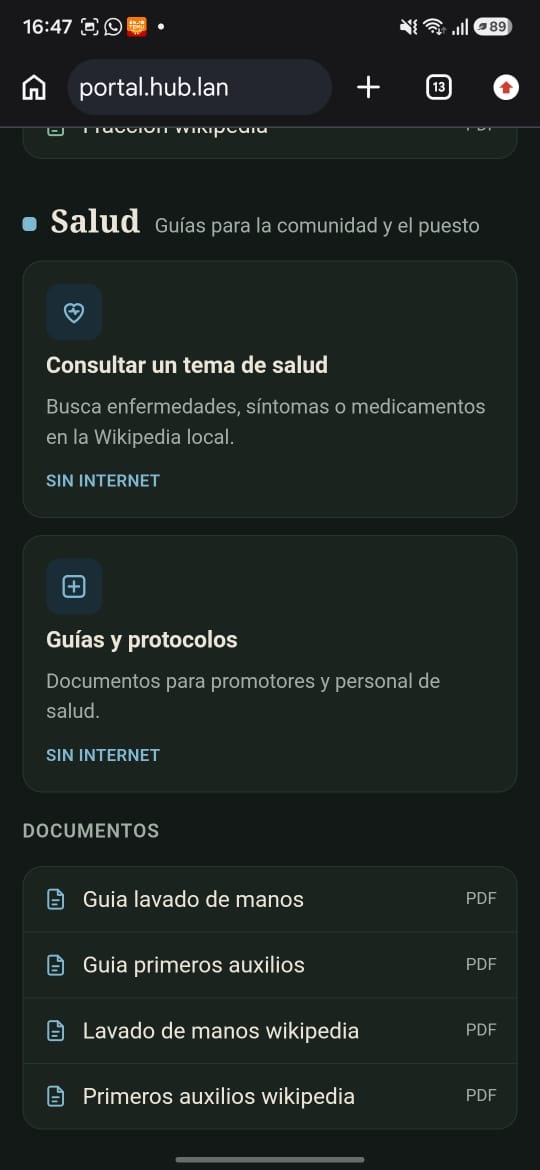
\includegraphics[width=0.32\columnwidth]{f23-p10-portal-salud.jpeg}\hfill

\includegraphics[width=0.32\columnwidth]{f23-p10-busqueda-wiki.jpeg}\hfill
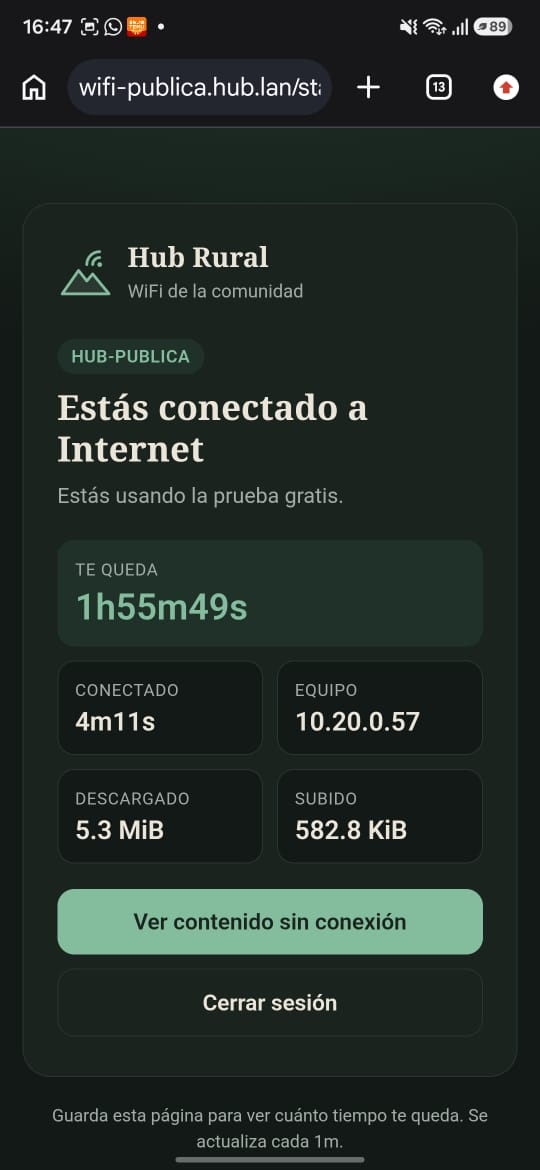
\includegraphics[width=0.32\columnwidth]{f23-hotspot-status.jpeg}
\caption{Celular en Hub-Publica: (izq.) sección Salud del portal con sus documentos; (centro) búsqueda de «volcán» en Kiwix; (der.) página de estado del Hotspot con la prueba gratis.}
\label{fig:celportal}
\end{figure}

\evid{f23-hotspot-activo-prueba.png}{Sesión de prueba del celular (\texttt{10.20.0.57}) en \texttt{/ip hotspot active} y su cola dinámica dentro de \texttt{publica}.}{fig:hsact}

Por último se pulió el portal (Figs.~\ref{fig:portal1}--\ref{fig:portal3}). La identidad visual toma el paisaje andino: una cabecera con cordilleras y un sol, y una paleta de verde páramo, verde guadua (Educación), azul río (Salud) y fucsia buganvilla (Ocio). Los títulos usan Bricolage Grotesque y el texto Atkinson Hyperlegible, diseñada para leerse bien con baja visión; ambas (licencia OFL) se alojan en el hub para que el portal no dependa de Internet. La búsqueda consulta Kiwix en formato XML (que Kiwix sirve con \texttt{Access-Control-Allow-Origin: *}) y muestra los artículos dentro del portal, con la palabra resaltada.

\evid{f23-portal-inicio.png}{Portal rediseñado: cabecera con el buscador, resumen del contenido y filtros por categoría con su número de elementos.}{fig:portal1}

\evid{f23-portal-busqueda.png}{Búsqueda de «energía»: los artículos de la Wikipedia sin conexión aparecen dentro del portal, con la palabra resaltada.}{fig:portal2}

\evid{f23-portal-autores.png}{Pie de página del portal con el proyecto, la asignatura y los autores.}{fig:portal3}

\subsection{Pruebas de caché y alta disponibilidad (P12 y P13)}
Para P12 se pidió dos veces el mismo archivo a través de Squid: la primera petición tardó 0,57~s y la segunda 0,002~s, y el contador \texttt{client\_http.hits} subió en uno (Fig.~\ref{fig:p12}). Squid~6 ya no agrega la cabecera \texttt{X-Cache}, por eso se usaron los contadores. Luego, con el celular en Hub-Publica, la misma página se sirvió desde la memoria (\texttt{TCP\_MEM\_HIT}) con la IP del celular, lo que confirma también el desvío transparente (Fig.~\ref{fig:p12cel}).

Para P13 se detuvo Squid. En menos de 10~s el \textit{netwatch} lo marcó caído y desactivó la regla \texttt{pbr-squid} (Fig.~\ref{fig:p13a}), y el celular siguió navegando por HTTP sin pasar por Squid (Fig.~\ref{fig:p13cel}). Al encenderlo, la regla se reactivó sola (Fig.~\ref{fig:p13b}).

\begin{figure*}[!t]\centering
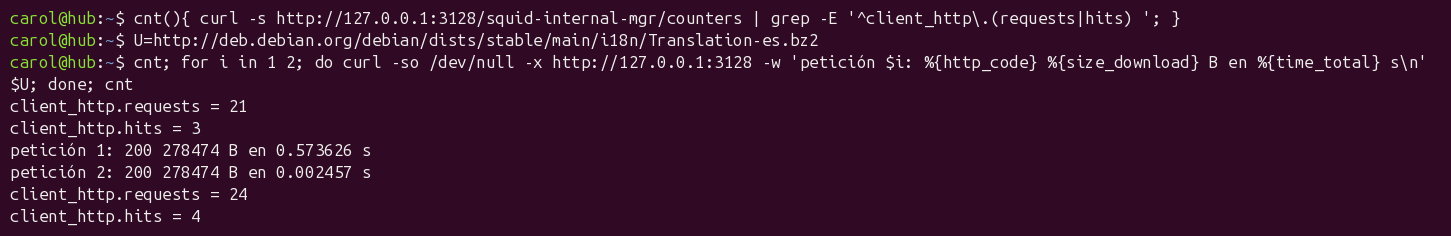
\includegraphics[width=0.85\textwidth]{f23-p12-squid-hit.png}\\[2pt]
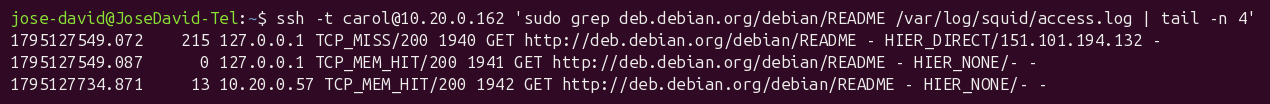
\includegraphics[width=\textwidth]{f23-p12-celular-log.png}
\caption{P12: (arriba) la segunda petición del mismo archivo sale de la caché de Squid (0,002~s) y sube el contador de aciertos; (abajo) registro de Squid con la petición del celular (\texttt{10.20.0.57}) servida como \texttt{TCP\_MEM\_HIT}.}
\label{fig:p12}\label{fig:p12cel}
\end{figure*}

\evid{f23-p13-pbr-desactivado.png}{P13: con Squid detenido, \textit{netwatch} lo detecta caído y la regla \texttt{pbr-squid} queda desactivada (X).}{fig:p13a}

\begin{figure}[!htbp]
\centering
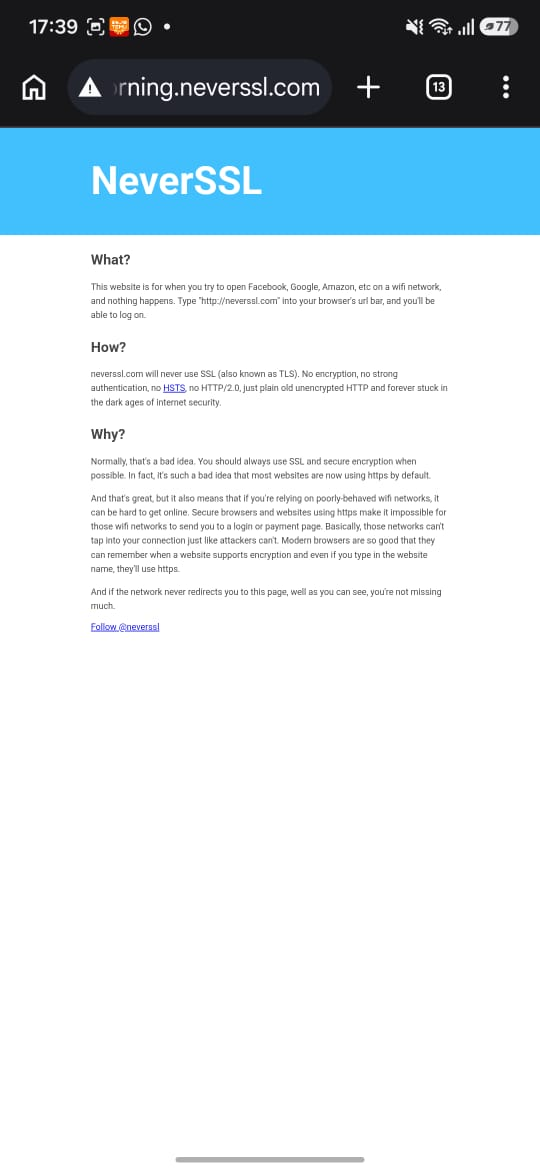
\includegraphics[width=0.40\columnwidth]{f23-p13-celular.jpeg}
\caption{P13: con Squid detenido, el celular sigue cargando un sitio por HTTP.}
\label{fig:p13cel}
\end{figure}

\evid{f23-p13-pbr-reactivado.png}{P13: al encender Squid, \textit{netwatch} vuelve a \texttt{up} y la regla \texttt{pbr-squid} se reactiva.}{fig:p13b}

\subsection{Starlink Mini: integración física y operación sin señal}
La Starlink Mini se conectó por su puerto RJ45 a \texttt{ether9} (Fig.~\ref{fig:fotosl}), en modo normal (sin \textit{bypass}, para no tener que restablecerla de fábrica al devolverla), y el portátil de administración pasó a \texttt{ether12}, donde recibió \texttt{10.20.0.171} por DHCP en la VLAN~10. Antes del cambio se guardó \texttt{hub-antes-starlink} (Fig.~\ref{fig:slantes}). El MikroTik recibió de la Mini \texttt{192.168.1.159/24} con puerta de enlace \texttt{192.168.1.1}; respondieron el router de la Mini y la antena (\texttt{192.168.100.1}), pero no \texttt{8.8.8.8}, porque dentro del laboratorio la antena no tuvo línea de vista al cielo (Fig.~\ref{fig:slint}). En modo normal hay triple traducción (MikroTik, router de la Mini y CGNAT); el \textit{bypass} la reduce a dos y queda para la instalación definitiva.

\begin{figure}[!htbp]
\centering
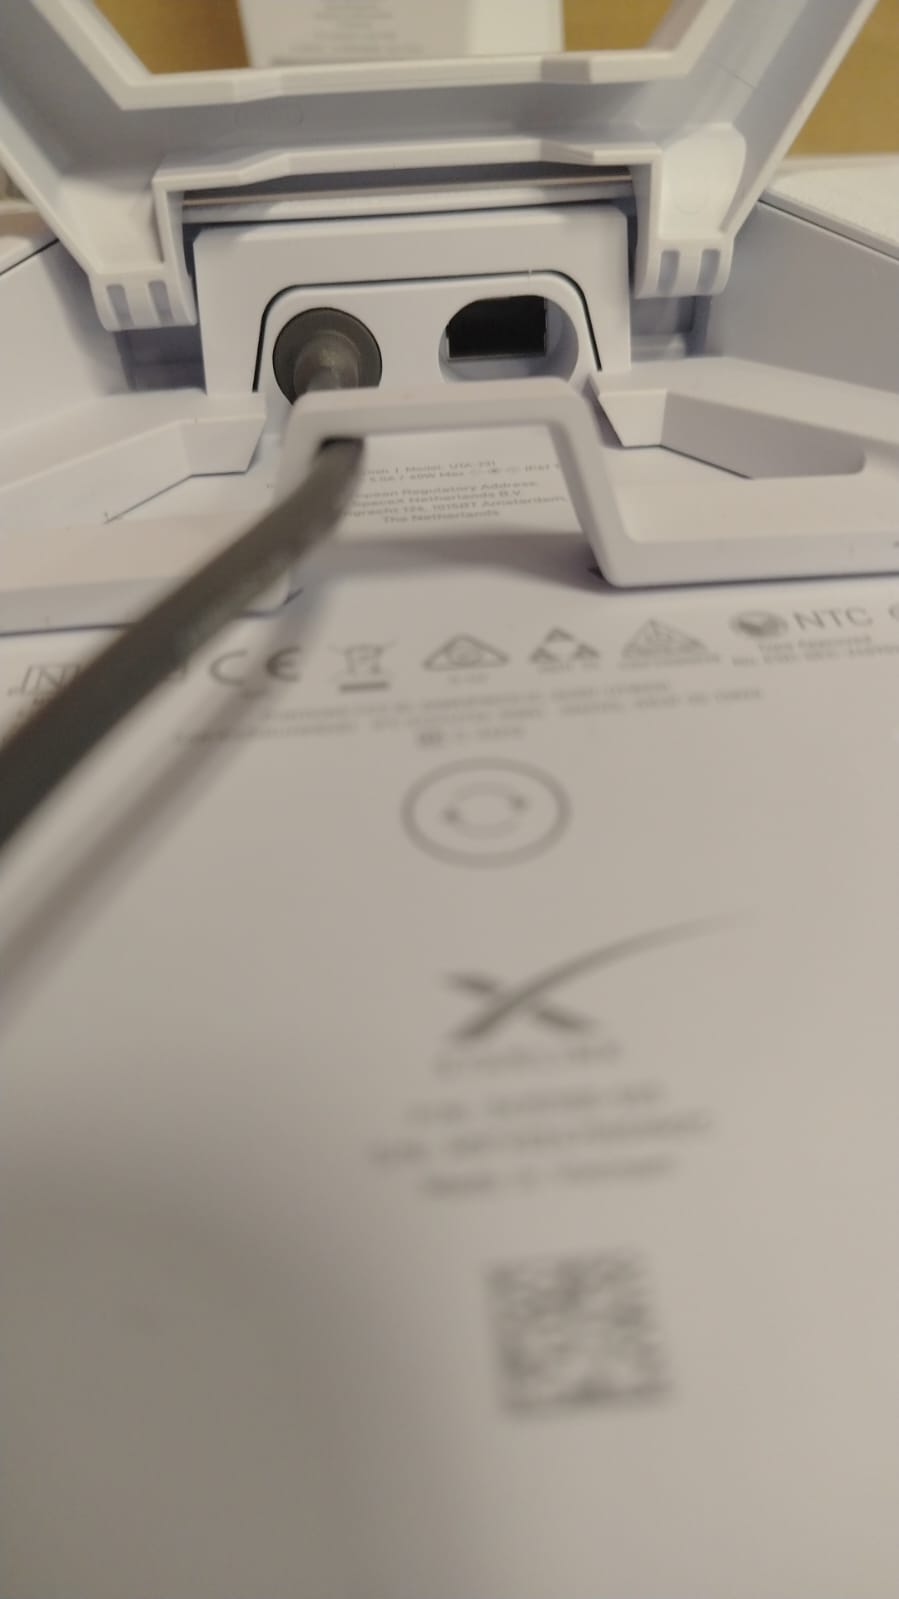
\includegraphics[width=0.45\columnwidth]{f23-foto-starlink.jpeg}
\caption{Starlink Mini conectada a \texttt{ether9} durante las pruebas en el laboratorio.}
\label{fig:fotosl}
\end{figure}

\evid{f23-starlink-antes.png}{Respaldo \texttt{hub-antes-starlink} y WAN por el portátil (\texttt{10.42.0.116}) antes del cambio.}{fig:slantes}

\evid{f23-starlink-integracion.png}{Starlink Mini en \texttt{ether9}: DHCP \texttt{192.168.1.159}, responden el router y la antena, pero no Internet (sin vista al cielo).}{fig:slint}

Esa situación es justamente el caso real del sitio sin señal, y sirvió como prueba sin conexión: el DNS local resolvió los nombres del hub (los de Internet no), y el portal, los PDF, las fuentes, la búsqueda de la Wikipedia y el tutorial respondieron 200 por HTTPS con certificado válido en 15--60~ms (Fig.~\ref{fig:offline}). La Raspberry mantuvo la hora, el MikroTik siguió sincronizado con ella, los cinco servicios siguieron activos y el DHCP siguió entregando direcciones (Fig.~\ref{fig:offhora}). Para lo que sí necesita Internet (paquetes, contenido), la WAN se simula con el portátil en la misma interfaz \texttt{ether9}: el MikroTik no nota la diferencia porque en ambos casos recibe la dirección por DHCP. Es una limitación del entorno de prueba, no del diseño.

\evid{f23-offline-starlink-sin-senal.png}{Hub sin Internet: DNS local, portal, PDF, fuentes, Wikipedia y tutorial en 200 por HTTPS.}{fig:offline}

\evid{f23-offline-hora-dhcp.png}{Hub sin Internet: hora mantenida, MikroTik sincronizado con la Raspberry, servicios activos y concesiones DHCP.}{fig:offhora}

%=====================================================================
\FloatBarrier
\section{Fase 2.4: CDN local de video}\label{sec:f24}
El 20/11/2026 se completó una CDN local de video en el disco USB del hub (\texttt{/srv/cdn/video/}), organizada en las mismas categorías del portal: \texttt{salud}, \texttt{educacion} y \texttt{ocio}.

% Las tablas de pruebas y de rúbrica se definen aquí para que LaTeX las ubique
% en la página de las secciones IX y XI y no después de las referencias.
\begin{table*}[!t]
\centering
\caption{Matriz de pruebas del prototipo físico y resultados}
\label{tab:pruebas}
\scriptsize
\begin{tabularx}{\textwidth}{lP{2.1cm}P{4.2cm}Yl}
\toprule
\textbf{ID} & \textbf{Criterio} & \textbf{Qué se prueba} & \textbf{Resultado obtenido} & \textbf{Estado} \\
\midrule
P1 & Instalación y SO & Todo vuelve tras \texttt{sudo reboot} & 5 servicios \texttt{active}, \texttt{/srv/cdn} con \texttt{noatime}, videos disponibles & Cumple \\
P2 & Instalación y SO & Seguridad básica & \texttt{Permission denied (publickey)}; ufw activo en \texttt{eth0} (Fig.~\ref{fig:ufw}) & Cumple \\
P3 & Conectividad & DHCP por relay, red pública & IP en \texttt{.10--.126} (\texttt{10.20.0.57}, \texttt{10.20.0.64}), gw \texttt{.1}, DNS \texttt{.162} (Fig.~\ref{fig:cel}) & Cumple \\
P4 & Conectividad & DHCP por relay, red de salud & IP en \texttt{.135--.158} (\texttt{10.20.0.148}, \texttt{10.20.0.157}), gw \texttt{.129} (Fig.~\ref{fig:cel}) & Cumple \\
P5 & Conectividad & DNS local y caché de dnsmasq & \texttt{portal.hub.lan} $\rightarrow$ \texttt{.162}; 12~ms y luego 0~ms desde la caché & Cumple \\
P6 & Conectividad & Hora común & MikroTik \texttt{synchronized} con \texttt{10.20.0.162} (Fig.~\ref{fig:ntp}) & Cumple \\
P7 & Conectividad & Portal cautivo en Hub-Publica & La página de acceso aparece sola; con la prueba gratis se navega (Fig.~\ref{fig:celportal}) & Cumple \\
P8 & Conectividad & Portal con usuario en Hub-Salud & El usuario de salud inicia sesión y navega; sesión en \texttt{/ip hotspot active} & Cumple \\
P9 & Caché estática & HTTPS obligatorio & HTTP $\rightarrow$ 301 a HTTPS con certificado válido \texttt{*.hub.lan} (Figs.~\ref{fig:cert} y~\ref{fig:c3}) & Cumple \\
P10 & Caché estática & Contenido sin iniciar sesión & Portal, guías PDF, Wikipedia y videos abren (200) sin sesión del Hotspot & Cumple \\
P11 & Rendimiento offline & Operación sin Internet & DNS, portal, PDF, Wikipedia y video en 200 con la Starlink sin señal (Fig.~\ref{fig:offline}) & Cumple \\
P12 & Caché estática & Aceleración con Squid & 2.ª petición 0,57~s $\rightarrow$ 0,002~s; celular \texttt{TCP\_MEM\_HIT} (Figs.~\ref{fig:p12} y~\ref{fig:p12cel}) & Cumple \\
P13 & Caché estática & Squid caído no corta la navegación & \texttt{pbr-squid} se desactiva en $<$10~s y se reactiva sola (Figs.~\ref{fig:p13a}--\ref{fig:p13b}) & Cumple \\
P14 & Conectividad & Aislamiento entre VLAN & Desde Hub-Publica no abren el AP (\texttt{.163}) ni el MikroTik (\texttt{.161}) & Cumple \\
P15 & Conectividad & Límite de ancho de banda & Cola dinámica de 1/2~Mbps por usuario bajo \texttt{publica} (Fig.~\ref{fig:hsact}) & Cumple \\
\midrule
V1 & Streaming & Cabeceras HTTP de un MP4 & \texttt{200}, \texttt{video/mp4}, \texttt{Accept-Ranges: bytes} & Cumple \\
V2 & Streaming & Petición de rango (\texttt{-r 0-99}) & \texttt{206 Partial Content} & Cumple \\
V3 & Streaming & Celular en Hub-Publica sin Internet & Reproduce de inmediato y se puede adelantar sin congelarse & Cumple \\
V4 & Almacenamiento & Persistencia tras reinicio & \texttt{videos.html} y \texttt{/srv/cdn/video/} disponibles & Cumple \\
\bottomrule
\end{tabularx}
\end{table*}

\begin{table*}[!t]
\centering
\caption{Criterios de la rúbrica, evidencia y nivel alcanzado}
\label{tab:rubrica}
\scriptsize
\begin{tabularx}{\textwidth}{lP{2.5cm}YP{1.7cm}}
\toprule
\textbf{Fase} & \textbf{Criterio} & \textbf{Evidencia (y lo que falta)} & \textbf{Nivel} \\
\midrule
\multirow{3}{*}{1. Plan} & Arquitectura de red & Topología L2/L3 con roles definidos (Fig.~\ref{fig:topo}), VLSM y DHCP (Tabla~\ref{tab:vlsm}), matriz de tráfico (Tabla~\ref{tab:matriz}) y puertos por etapa (Tabla~\ref{tab:puertos}); router y servidor separados para no sobrecargar la RPi5 & Accomplished \\
 & Estrategia de caché & Jerarquía RAM/NVMe/SSD, presupuesto del disco, \texttt{refresh\_pattern} por tipo, \texttt{heap LFUDA} y HTTPS sin descifrar (Sección~\ref{sec:jose}), aplicados en Squid (Sección~\ref{sec:f23}) & Accomplished \\
 & Cronograma y recursos & Cronograma de 11 semanas con ruta crítica, compras en tres lotes con contingencia y matriz de 12 riesgos (corte eléctrico y falta de enlace como los mayores) & Accomplished \\
\midrule
\multirow{3}{*}{2. Prototipo} & Instalación y SO & Ubuntu Server 24.04 con servicios estables en systemd; ext4 con \texttt{noatime,nofail}, inodos para archivos grandes y SMART; ufw restrictivo, SSH solo con llave y \texttt{unattended-upgrades}; todo vuelve tras reiniciar (P1, P2). El prototipo usa un disco de 465~GB; el de 2--4~TB es de la Fase~3 & Accomplished \\
 & Caché de contenido estático & Squid transparente con conmutación por \textit{netwatch}, Nginx HTTPS, PDF por categoría y Wikipedia sin conexión (P9--P13) & Accomplished \\
 & Conectividad local & DHCP por relay a las tres VLAN, DNS \texttt{hub.lan} con caché, Hotspot por VLAN con \textit{walled garden}, aislamiento y colas (P3--P8, P14, P15) & Accomplished \\
\midrule
\multirow{4}{*}{3. Operación} & Streaming de video & Video 720p fluido sin conexión con peticiones de rango y \textit{faststart} (V1--V4). Sin Jellyfin ni transcodificación en vivo, por la decisión de la Sección~\ref{sec:f24} & Proficient \\
 & Gestión de almacenamiento & Directorios por servicio y categoría (\texttt{www/pdf/<cat>}, \texttt{video/<cat>}, \texttt{kiwix}), caché de Squid con tope y reemplazo LFUDA, \texttt{nofail} y \texttt{RequiresMountsFor}. Falta: cuotas y purga automática del contenido viejo & Proficient \\
 & Interfaz de usuario & Portal con categorías Educación, Salud y Ocio, búsqueda local sin tildes, búsqueda de la Wikipedia integrada y catálogo de video (Figs.~\ref{fig:portal1}--\ref{fig:portal3}) & Accomplished \\
 & Rendimiento y modo desconectado & Todo el contenido local funciona sin Internet (P11, V3) y Squid se omite solo si cae (P13). Falta: \texttt{offline\_mode} de Squid y sincronización automática al volver el enlace & Proficient \\
\bottomrule
\end{tabularx}
\end{table*}

\subsection{Perfil de codificación}
Los videos se procesan una sola vez, antes de cargarlos, con ffmpeg~\cite{ffmpeg}: MP4 con H.264 y audio AAC estéreo a 96~kbps, escalados a 720p con tasa máxima de 1,2~Mbps (\texttt{-crf 26 -maxrate 1200k -bufsize 2400k}) y la opción \texttt{-movflags +faststart}. El perfil responde a tres criterios:
\begin{itemize}
\item \textbf{Compatibilidad:} H.264/AAC en MP4 se reproduce en cualquier navegador móvil (Android e iOS) sin instalar aplicaciones.
\item \textbf{Ajuste a las colas:} con $\approx$1,3~Mbps entre video y audio, la reproducción cabe en la cola de 2~Mbps por usuario y en los 20~Mbps del grupo de Hub-Publica, sin cortes.
\item \textbf{Inicio inmediato:} \textit{faststart} pone el índice (\textit{moov atom}) al inicio del archivo, así el navegador empieza a reproducir con los primeros bytes en lugar de esperar el archivo completo.
\end{itemize}

\textbf{Decisión: sin Jellyfin ni transcodificación en vivo.} La Raspberry Pi~5 no tiene codificador H.264 por hardware, y transcodificar en su CPU para varios celulares a la vez la saturaría y le quitaría recursos al DNS, al DHCP y a Squid. Como el contenido es fijo y se carga desde la sede, es más eficiente codificarlo una vez en un equipo externo y servirlo como archivo estático: la Pi solo lee del disco y envía bytes.

\subsection{Servicio en Nginx con peticiones de rango}
Nginx publica el directorio con este bloque, dentro del servidor HTTPS del portal:
\begin{lstlisting}
location ^~ /video/ {
    alias /srv/cdn/video/;
    autoindex on;
    expires 7d;
}
\end{lstlisting}
El prefijo \texttt{\textasciicircum\textasciitilde} le da prioridad sobre la expresión regular de archivos estáticos del portal, que de otro modo capturaba las miniaturas \texttt{.jpg} de los videos y devolvía 404. Nginx atiende las peticiones de rango de HTTP~\cite{rfc9110}: ante \texttt{Range: bytes=...} responde \texttt{206 Partial Content} con solo ese fragmento, de modo que el usuario puede pausar y adelantar el video sin descargarlo completo ni transcodificar en el servidor.

\subsection{Catálogo web}
El script \texttt{generar-videos.sh} recorre las categorías, toma la miniatura \texttt{.jpg} de cada video y genera \texttt{/srv/cdn/www/videos.html} con etiquetas HTML5 \texttt{<video controls preload="metadata">}, enlazada desde el portal. Con \texttt{preload="metadata"} el celular solo descarga el encabezado hasta que el usuario presiona reproducir, lo que ahorra ancho de banda del Wi-Fi.

\subsection{Pruebas}
\begin{itemize}
\item \textbf{V1:} la cabecera (\texttt{HEAD}) de un MP4 devuelve \texttt{200}, \texttt{video/mp4} y \texttt{Accept-Ranges: bytes}.
\item \textbf{V2:} una petición de rango (\texttt{curl -r 0-99}) devuelve \texttt{206 Partial Content}.
\item \textbf{V3:} en un celular en Hub-Publica, sin Internet, el video empieza de inmediato y se puede adelantar sin congelarse.
\item \textbf{V4:} tras reiniciar la Raspberry, el catálogo y el directorio de video siguen disponibles.
\end{itemize}

%=====================================================================
\section{Evaluación experimental}
La Tabla~\ref{tab:pruebas} consolida las pruebas del prototipo físico: las 15 de red y servicios (P1--P15) y las 4 de video (V1--V4), cada una asociada a un criterio de la rúbrica y a su evidencia.


%=====================================================================
\section{Problemas resueltos en las Fases 2.3 y 2.4}
\begin{itemize}
\item \textbf{Servicios caídos al arrancar:} \texttt{/etc/fstab} tenía dos montajes con la etiqueta \texttt{HUBDATA} en \texttt{/srv/cdn} (el disco USB y un archivo de 10~GB de reemplazo), y el contenido estaba solo en el archivo. Se copió al disco USB y se dejó una sola línea activa.
\item \textbf{Fecha incorrecta en la Raspberry:} no tiene RTC con pila y arrancó sin Internet, así que el certificado aparecía como aún no válido y el MikroTik quedaba en \texttt{waiting}. Se reinició chrony con Internet; la solución definitiva (pila del RTC) queda para la Fase~3.
\item \textbf{Comandos de varias líneas por SSH fallan en RouterOS:} cada línea pierde el menú; se escribe la ruta completa en cada comando.
\item \textbf{SSH aceptaba contraseña:} tras un acceso de emergencia, \texttt{PasswordAuthentication} quedó en \texttt{yes}; se volvió a \texttt{no} y se verificó con P2.
\item \textbf{SSH colgado tras activar ufw:} faltaba la regla del portátil; se agregó desde la consola local.
\item \textbf{El portátil no veía la web del AP:} el AP solo responde a su red; se usó un NAT de laboratorio que se borra al cerrar.
\item \textbf{Enlace intermitente en \texttt{ether9}:} cable flojo; se cambió y se repitió la ruta hacia la red del hub.
\item \textbf{La ruta del portátil hacia el hub desaparecía:} NetworkManager la borra cada vez que reinicia la conexión compartida. Se resolvió pasando el portátil a \texttt{ether12}, donde recibe IP por DHCP en la VLAN~10.
\item \textbf{Proyecto Gutenberg no disponible desde la red del laboratorio (503):} las fábulas se tomaron de Wikisource en español, con reintentos y caché local porque limita las consultas seguidas (429).
\item \textbf{Miniaturas de video con 404:} la expresión regular de estáticos de Nginx tenía prioridad sobre \texttt{/video/}; se resolvió con \texttt{location \textasciicircum\textasciitilde{} /video/}.
\item \textbf{Espera al iniciar el video en el celular:} el índice del MP4 estaba al final; se movió al inicio con \texttt{-movflags +faststart}.
\end{itemize}

%=====================================================================
\section{Evaluación frente a la rúbrica}
La Tabla~\ref{tab:rubrica} relaciona cada criterio de las tres fases de la rúbrica con la evidencia de este informe y el nivel que el equipo considera alcanzado, con lo que falta para el nivel más alto cuando aplica.


\subsection{Trabajo futuro}
\begin{itemize}
\item SSD de 2~TB definitivo con la distribución del presupuesto de la Fase~1, y caché de Squid de 50--100~GB.
\item Script de purga (\texttt{systemd timer}) que borre los videos y documentos más antiguos o menos vistos cuando el disco pase de un umbral, y cuotas por categoría.
\item Conmutación online/offline: un \textit{heartbeat} con histéresis que active \texttt{offline\_mode} en Squid y lance la sincronización de contenido una vez por conexión, con avisos por MQTT.
\item Pila del RTC (\texttt{dtparam=rtc\_bbat\_vchg}) para tener hora correcta sin Internet tras cada apagado.
\item Batería con medición de consumo, autonomía y apagado ordenado al 15~\%.
\item Starlink en modo \textit{bypass} con el UniFi UAP-AC-M definitivo, y retiro de las reglas de laboratorio.
\item Certificado real con Let's Encrypt por DNS-01 y CA de pruebas restringida a \texttt{hub.lan} (\texttt{nameConstraints}), porque la actual podría firmar certificados para cualquier dominio si se filtrara su llave.
\end{itemize}

%=====================================================================
\section{Conclusiones}
El diseño consolidado funciona en hardware físico. Separar el enrutamiento, el portal cautivo, el relay y las colas en el MikroTik de los servicios en la Raspberry Pi~5 hizo que los cambios y fallas de las aplicaciones no afectaran la conectividad de capas 2 y 3, como mostró la prueba con Squid apagado. La segmentación en tres VLAN, con un SSID y un perfil de portal por grupo, el firewall y las colas cumplen el requisito de redes independientes por grupo de interés.

El enfoque \textit{offline-first} quedó validado en el escenario real: con la Starlink conectada pero sin señal, los usuarios siguieron teniendo nombres locales, hora, portal, guías de salud, Wikipedia y video. Codificar el video una vez, con tasa limitada e índice al inicio, y servirlo con peticiones de rango permitió reproducción inmediata en celulares sin cargar la CPU de la Raspberry y dentro de la política de colas.

Validar primero en GNS3 y llevar los equipos a lo físico uno a la vez permitió aislar cada falla, y guardar un \texttt{/export} después de cada cambio permitió recuperar el estado en minutos. Lo pendiente para la operación en campo (disco definitivo, purga automática, conmutación online/offline y energía) no exige cambiar el diseño, solo ampliarlo.

\subsection*{Repositorio}
Configuraciones, scripts, capturas y bitácoras: \url{https://github.com/JOSED235/ProyectoRedesRurales}.

\begin{thebibliography}{00}
\bibitem{ieee8021q} IEEE, ``IEEE Standard for Local and Metropolitan Area Networks -- Bridges and Bridged Networks,'' IEEE Std 802.1Q-2018.
\bibitem{rfc1918} Y. Rekhter \textit{et al.}, ``Address Allocation for Private Internets,'' BCP 5, RFC 1918, Feb. 1996.
\bibitem{dnsmasq} S. Kelley, ``dnsmasq documentation,'' \url{https://thekelleys.org.uk/dnsmasq/doc.html} (accedido el 16 oct. 2026).
\bibitem{squid} Squid Web Proxy Cache, ``Configuration Reference,'' \url{http://www.squid-cache.org/Doc/config/} (accedido el 16 oct. 2026).
\bibitem{nginx} Nginx, ``Documentation,'' \url{https://nginx.org/en/docs/} (accedido el 16 oct. 2026).
\bibitem{kiwix} Kiwix, ``Offline Internet content,'' \url{https://kiwix.org/} (accedido el 16 oct. 2026).
\bibitem{who-hh} World Health Organization, \textit{WHO Guidelines on Hand Hygiene in Health Care}. Geneva: WHO, 2009.
\bibitem{ifrc-fa} International Federation of Red Cross and Red Crescent Societies, \textit{International First Aid, Resuscitation, and Education Guidelines 2020}. Geneva: IFRC, 2020.
\bibitem{rfc9110} R. Fielding, M. Nottingham y J. Reschke, ``HTTP Semantics,'' RFC 9110 (STD 97), Jun. 2022, Sec. 14 (Range Requests; reemplaza a RFC 7233).
\bibitem{ffmpeg} FFmpeg Developers, ``FFmpeg Documentation,'' \url{https://ffmpeg.org/ffmpeg.html} (accedido el 20 nov. 2026).
\end{thebibliography}

\end{document}
